\documentclass[usenames,dvipsnames]{beamer}
\usepackage[utf8]{inputenc}
\usepackage{verbatim}
\usetheme{uniud}


%: Portada {{{
%%% Some useful commands
% pdf-friendly newline in links
\newcommand{\pdfnewline}{\texorpdfstring{\newline}{ }} 
% Fill the vertical space in a slide (to put text at the bottom)
\newcommand{\framefill}{\vskip0pt plus 1filll}


\title[SDK Android para Comunicar con Redes Blockchain]{\LARGE Diseño e Implementación de un SDK Android para Facilitar la Interacción de Aplicaciones Móviles con una Blockchain}
\date[Jun 2021]{Jun 17, 2021}
\author[Jorge Sol Gonzalez]{
  Jorge Sol Gonzalez, TFG
  \pdfnewline
  \texttt{jorgesolgonzalez1998@gmail.com}
}
\institute{ETSI Informáticos, Universidad Politécnica de Madrid}

\begin{document}

\begin{frame}
\titlepage
\end{frame}

\begin{frame}
\frametitle{Índice} 
\tableofcontents
\end{frame}
%: }}}


%: Indice {{{
%%% Cosas de valor
% A minuto por transparencia
% Poner en valor lo que hemos hecho
% TryIT y Taller de Machine Learning
% Curva de aprendizage grande

%%% Índice
% Hola e Indice ==> 1:00
% Motivación y Objetivos ==> 1:30
%   Qué es Estublock?
%   Objetivos del Proyecto (objetivos de forma genérica)
% Tecnología Actual ==> 2:30
%   Qué es Blockchain?
%   Aplicaciones Móviles con Blockchain
%   Hablar de android de forma nativa vs hibridas y por que he elegido android + añadir web3j
%%% --> 5 minutos hasta aquí
% Desarrollo Móvil ==> 5:00
%   Casos de Uso
%   Interfaz de Usuario % Explicar problrma con androidstudio
%   Librerías Principales (equilibrio sin entrar en demasiado detalle, número de librerias o lineas de código)
% SDK ==> 4:00
%   Diseño del SDK % diagrama para mostrar como esta formado 
%   Seguridad y Keystore
%   Uso y Documentación
% Una diapo global para la DEMO? 
% DEMO ==> 1:30 (vídeo con 2 móviles y por eso es un vídeo)
% Conclusiones y Trabajo Futuro ==> 1:30
%   Conclusiones (madurez de las herramientas, resultados, que has aprendido, que te ha permitido, ideas extraidas, falta de librerías especificas, blockchain es una realidad (estado de madurez de la tecnología))
%   Impacto Ambiente
%   Trabajo Futuro
%%%
%: }}}


%: Motivacion y Objetivos {{{
\section{Motivación y Objetivos}
\begin{frame} 
\frametitle{¿Qué es Estublock?} 
  \begin{center}
    
\includegraphics[scale=0.50]{graphics/logo_catedra}
  \end{center}
  \begin{center}
    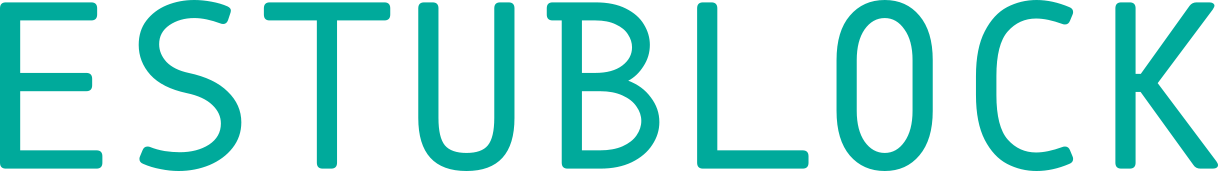
\includegraphics[scale=0.25]{graphics/texto_estublock}
  \end{center}
\end{frame}

\begin{frame} 
\frametitle{Motivación} 
  \begin{block}{Motivación}
    \begin{itemize}
      \item Mejorar el sistema de listas de asistencias a eventos.
      \item Implantar un sistema común para el registro de alumnos a estos eventos.
      \item Crear un sistema fiable y seguro de acreditación de asistencias.
      \item Herramienta de código abierto para el resto de universidades.
    \end{itemize}
  \end{block} 
\end{frame}

% Objetivos de forma genérica
\begin{frame} 
\frametitle{Objetivos del Proyecto} 
  \begin{block}{Objetivos}
    \begin{itemize}
      \item Analizar la tecnología Blockchain y librerías existentes
      \item Desarrollo de una aplicación móvil que resuelva el problema planteado
      \item Desarrollo de un SDK para facilitar las llamadas a la red Blockchain
      \item Redactar una documentación para futuros desarrolladores
    \end{itemize}
  \end{block}
\end{frame}
%: }}}


%: Tecnología Actual {{{
\section{Tecnología Actual}
\begin{frame} 
\frametitle{¿Qué es Blockchain?} 
  \begin{columns}
  \begin{column}{0.5\textwidth}
    \center \textcolor{UniGold}{\emph{Distributed Ledger Tecnology}}
    \begin{itemize}
      \item Transparencia
      \item Inmutabilidad
      \item Descentralización
    \end{itemize}
  \end{column}
  \begin{column}{0.5\textwidth}
    \begin{tikzpicture}
      \node[inner sep=0pt] (logo) at (12,6){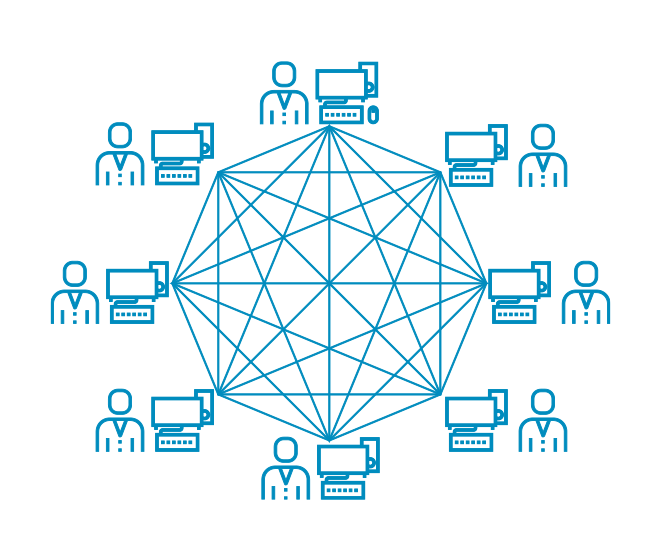
\includegraphics[scale=0.25]{graphics/blackchain}};
      \node[inner sep=0pt] (logo) at (12,2.3){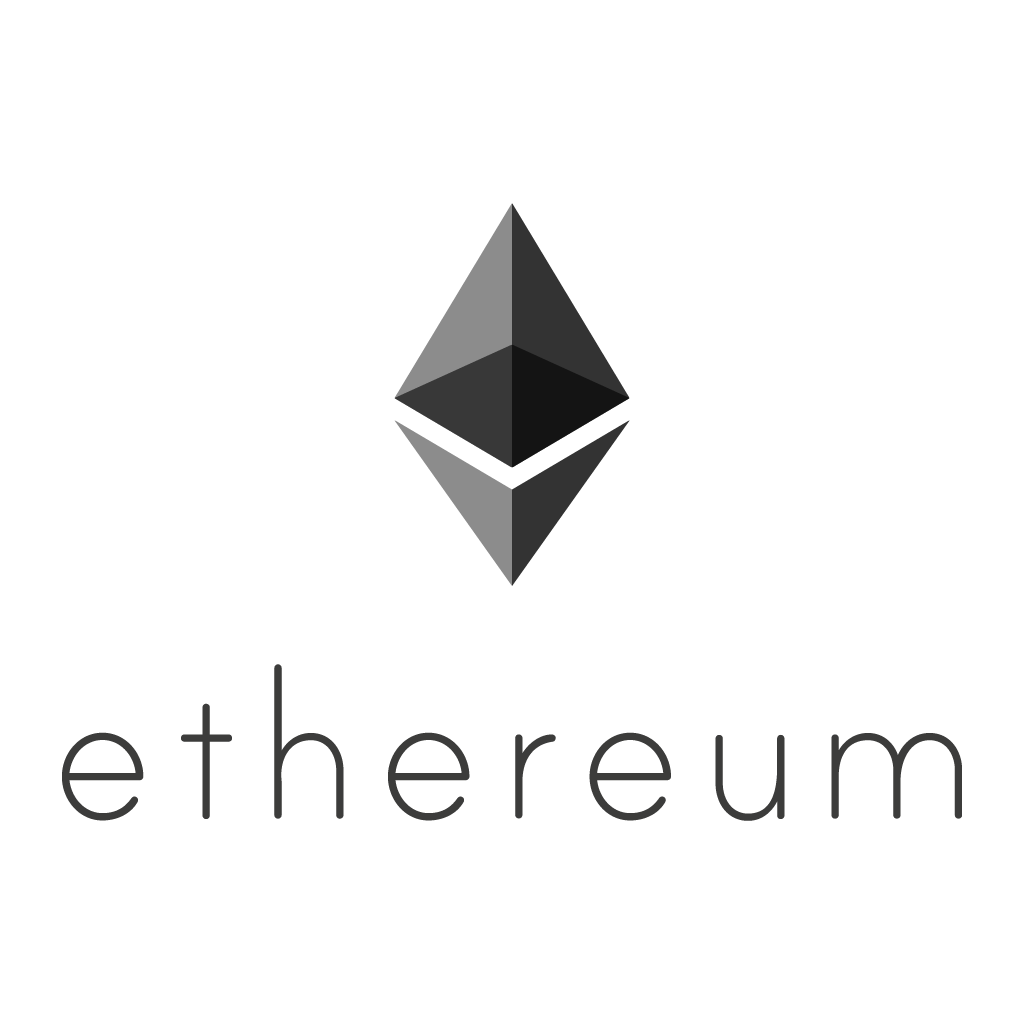
\includegraphics[scale=0.20]{graphics/logo_ethereum}};
    \end{tikzpicture}
  \end{column}
  \end{columns}
\end{frame}

\begin{frame} 
\frametitle{Aplicaciones Móviles con Blockchain} 
  \begin{columns}
  \begin{column}{0.6\textwidth}
    \center \textcolor{UniGold}{Aplicaciones Distribuidas (DApps)}
    \begin{itemize}
      \item \textcolor{UniGold}{\small GUTS:} Plataforma que registra entradas a conciertos, teatros, eventos, etc
      \item \textcolor{UniGold}{lifeID:} Plataforma de identidad digital
      \item \textcolor{UniGold}{Voatz:} Plataforma electoral
    \end{itemize}
  \end{column}
  \begin{column}{0.4\textwidth}
    \begin{tikzpicture}
      \node[inner sep=0pt] (logo) at (0,7){
\includegraphics[scale=0.08]{graphics/logo_guts}};
      \node[inner sep=0pt] (logo) at (0,5){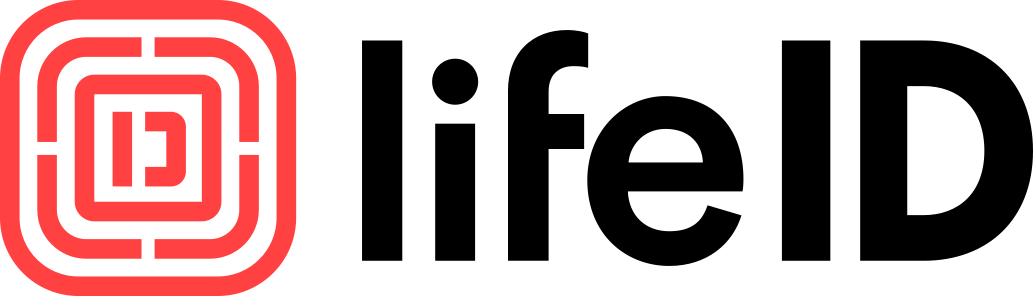
\includegraphics[scale=0.125]{graphics/logo_lifeid}};
      \node[inner sep=0pt] (logo) at (0,3){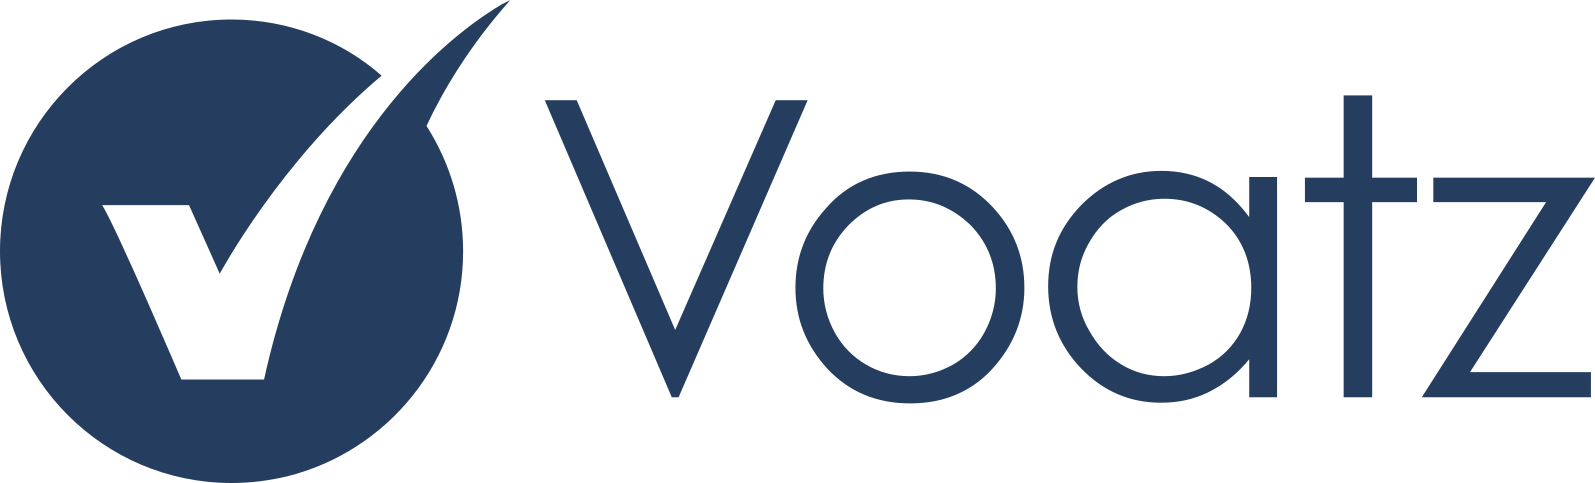
\includegraphics[scale=0.08]{graphics/logo_voatz}};
    \end{tikzpicture}
  \end{column}
  \end{columns}
\end{frame}

% Por qué he elegido aplicación nativa de Android y no una hibrida (mirar si hay web3j para hibridas)
\begin{frame} 
\frametitle{¿Por qué Android?}
  \begin{columns}
  \begin{column}{0.6\textwidth}
    \center \textcolor{UniGold}{Tipos de aplicaciones}
    \begin{itemize}
      \item Nativas
      \item Web
      \item Híbridas
    \end{itemize}
    \pause
    \center \textcolor{UniGold}{Sistemas Operativos}
    \begin{itemize}
      \item Cuota de \textbf{Android} \emph{86.1\%}
      \item Cuota de \textbf{iOS} \emph{13.9\%}
      \item Otros: Windows Phone, BlackBerry, Google Nexus, etc
    \end{itemize}
  \end{column}
  \begin{column}{0.4\textwidth}
    \begin{tikzpicture}
      \node[inner sep=0pt] (logo) at (0,6.5){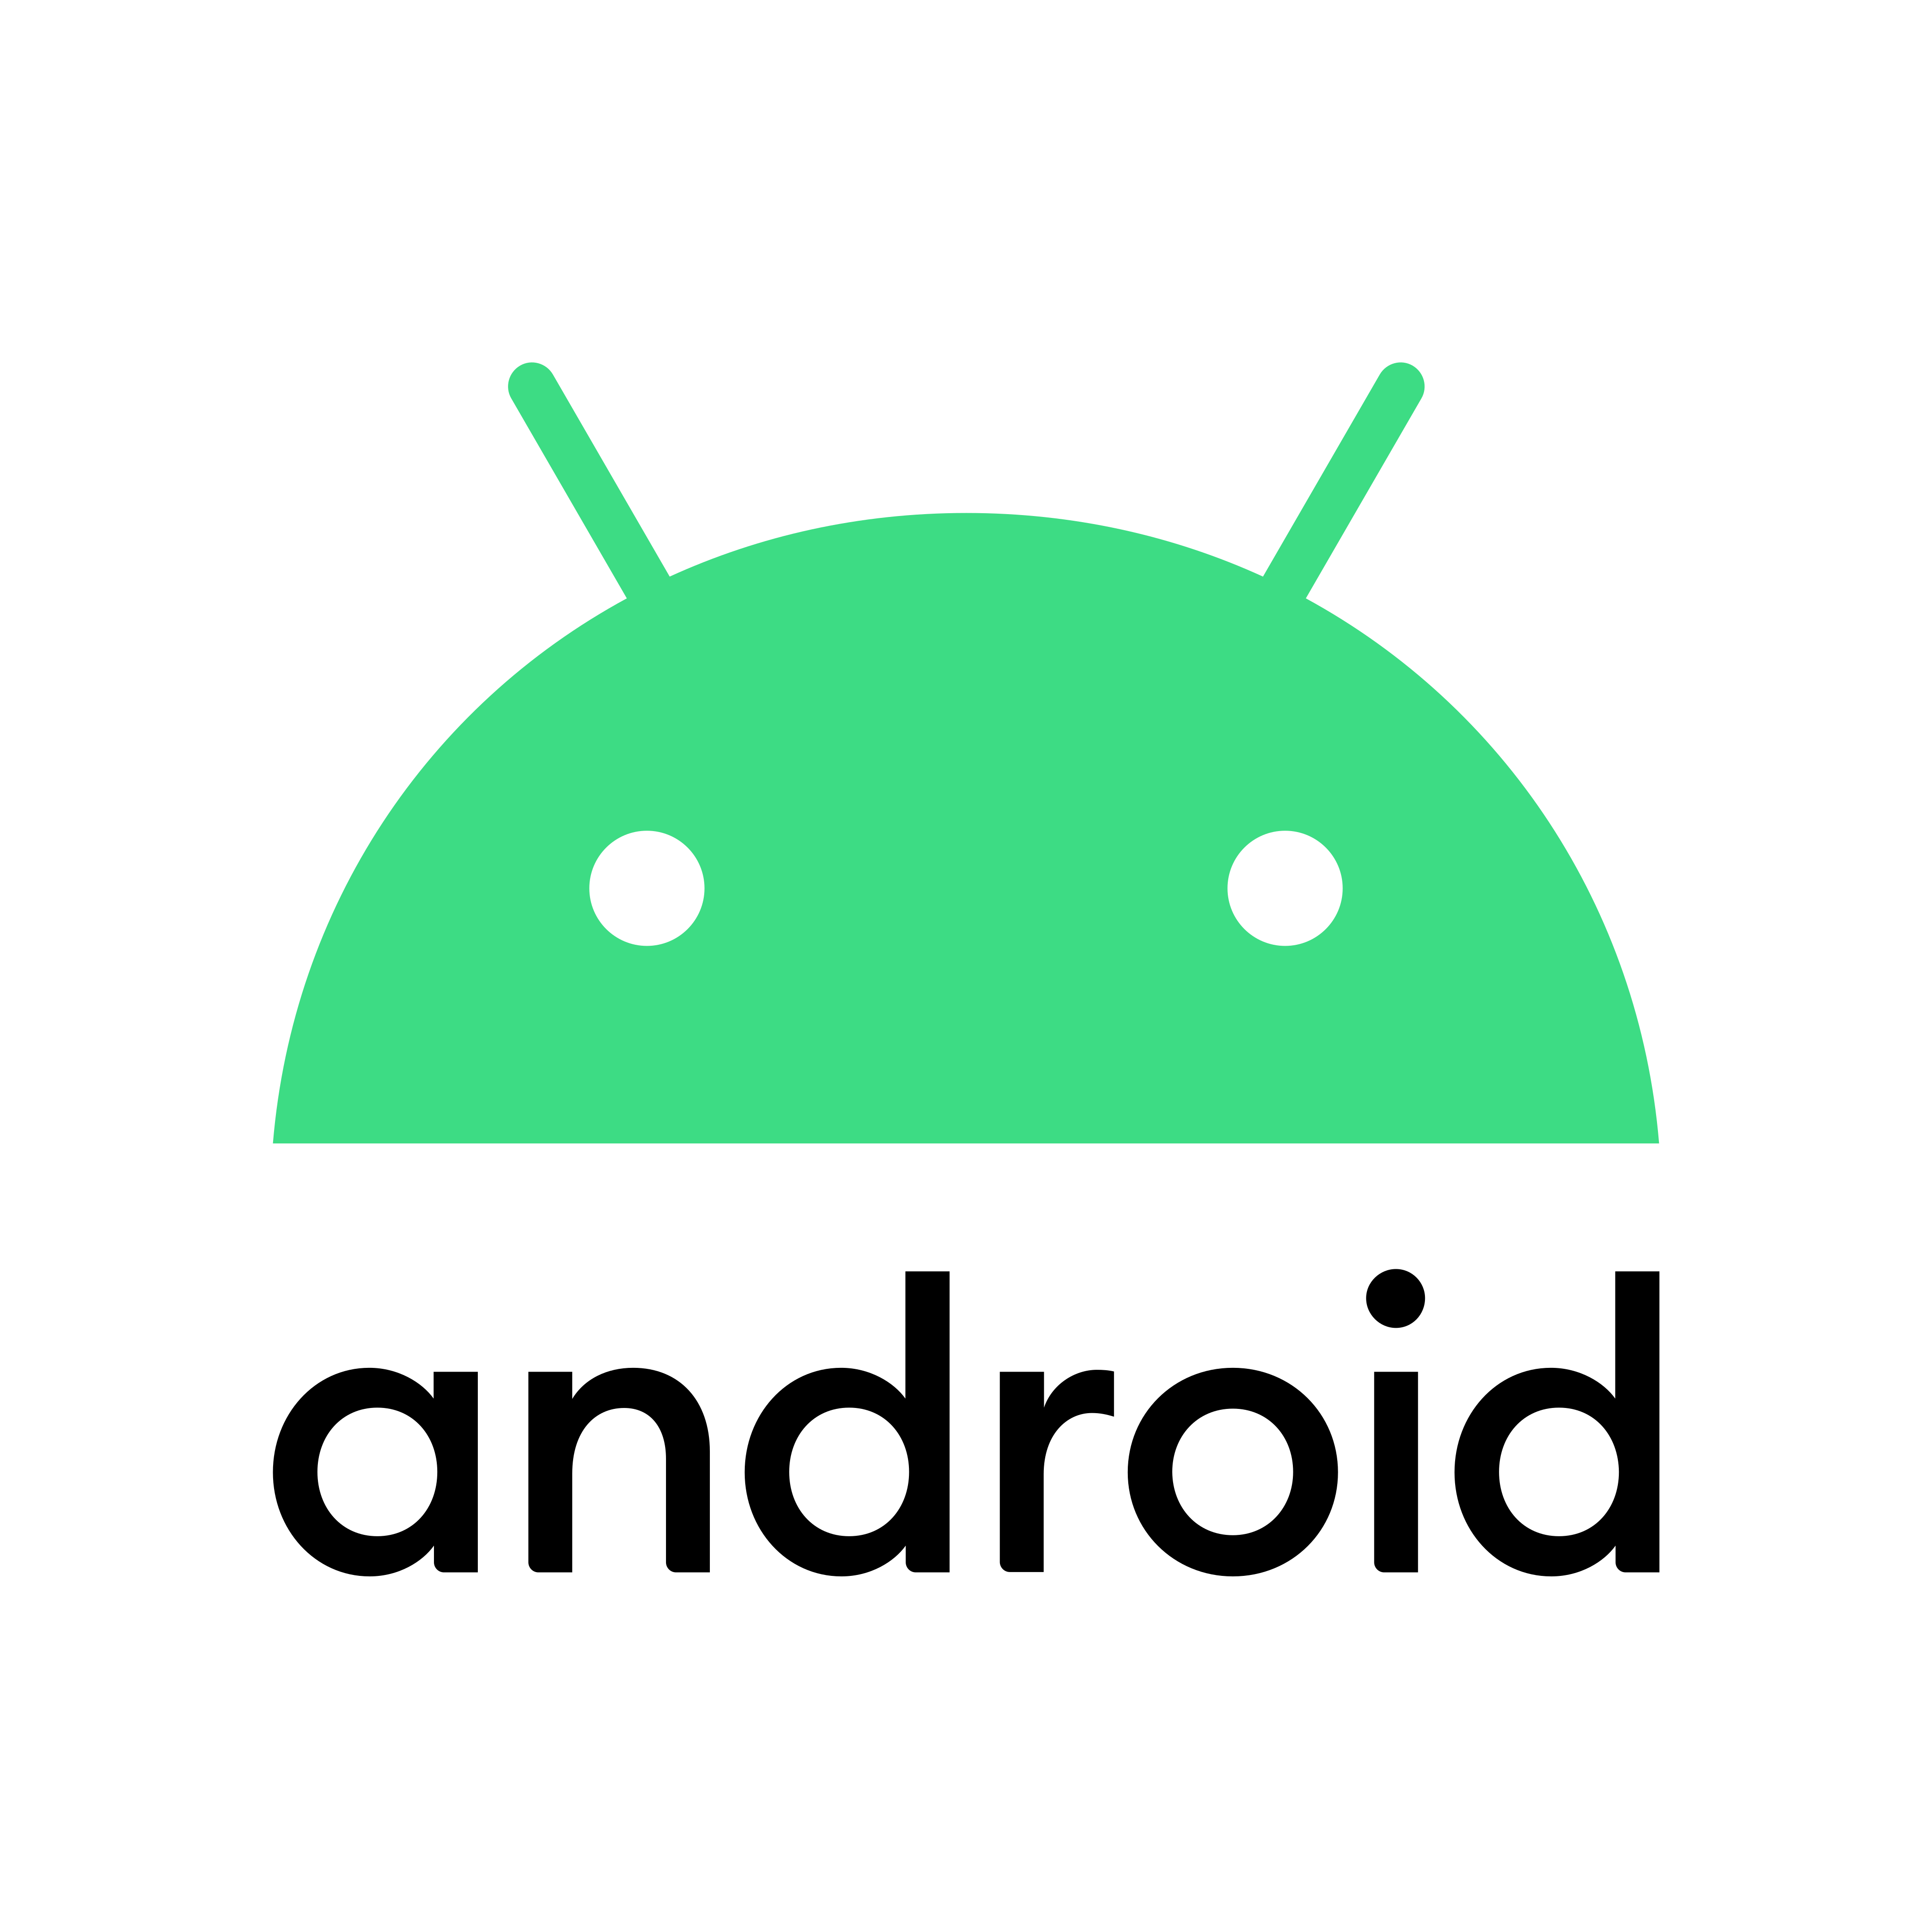
\includegraphics[scale=0.04]{graphics/logo_android}};
      \node[inner sep=0pt] (logo) at (0,3.5){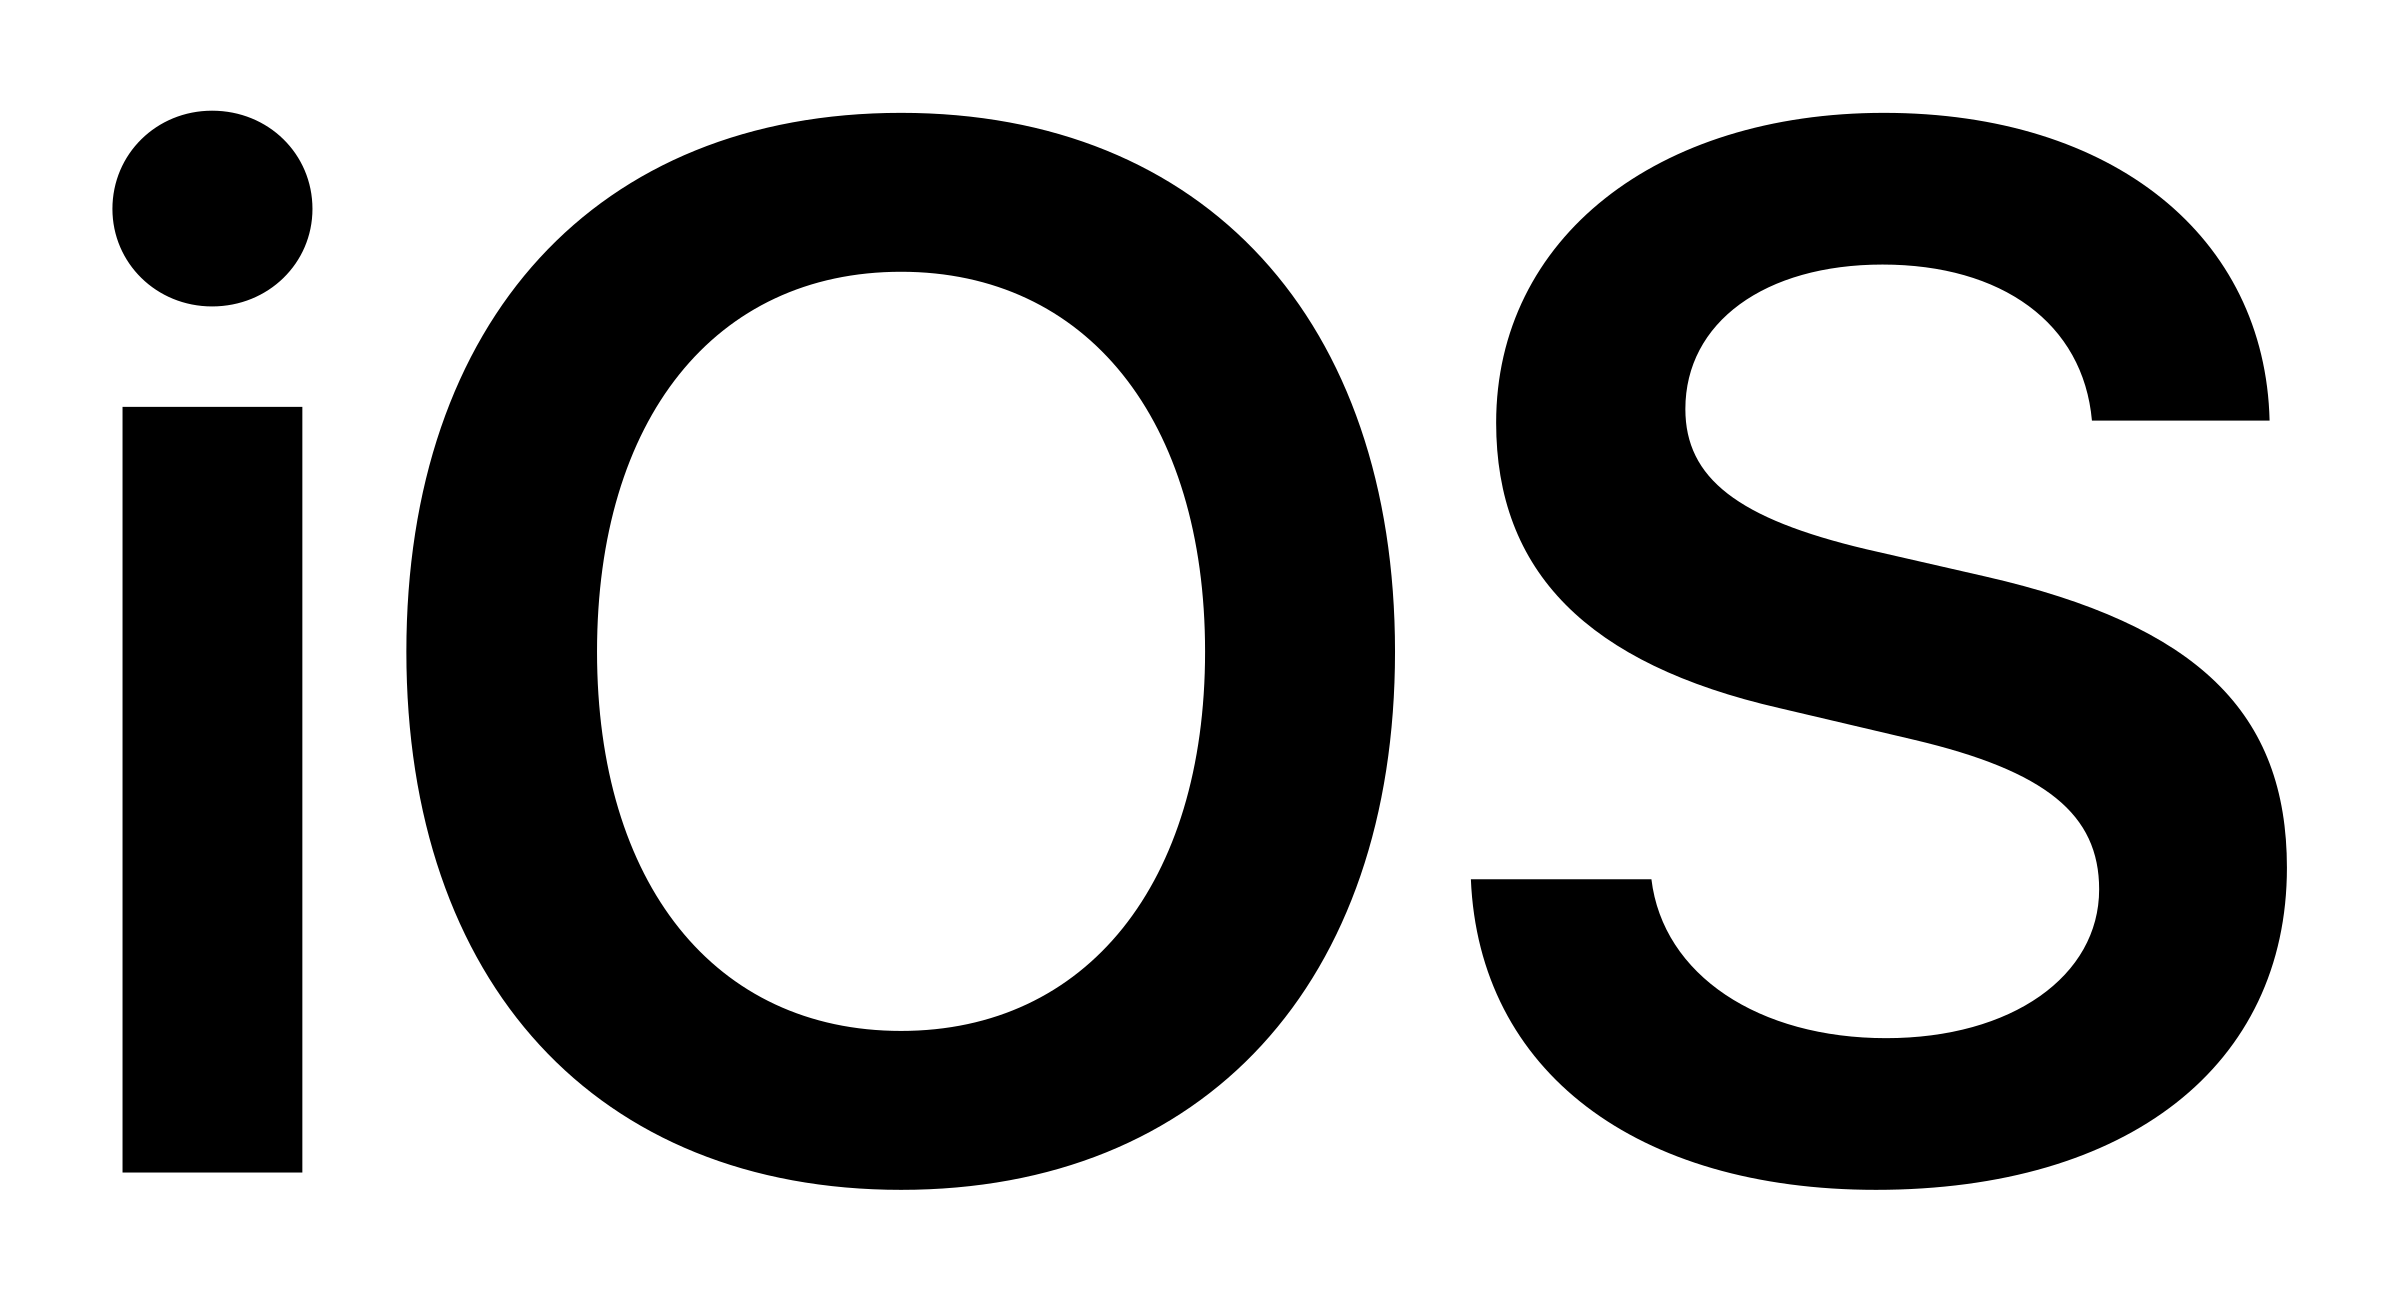
\includegraphics[scale=0.80]{graphics/logo_apple}};
    \end{tikzpicture}
  \end{column}
  \end{columns}
\end{frame}
%: }}}


%: Desarrollo Móvil {{{
\section{Desarrollo Móvil}
\begin{frame} 
\frametitle{Casos de Uso} 
  \begin{block}{Casos de Uso de Estublock}
     \begin{itemize}
      \item Login
      \item Registro
      \item Suscripción a un tema
      \item Eliminar suscripción a un tema
      \item Generar QR
      \item Escanear QR
    \end{itemize}
  \end{block}
\end{frame} 

\begin{frame} 
\frametitle{Casos Uso General} 
  \begin{center}
  \begin{tikzpicture}
    \node[inner sep=0pt] (logo) at (0,5){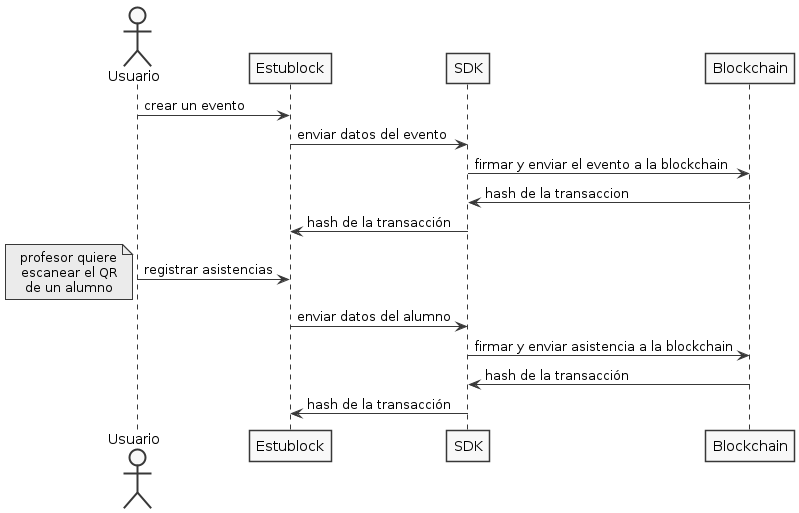
\includegraphics[scale=0.35]{graphics/uml_presentacion}};
  \end{tikzpicture}
  \end{center}
\end{frame}

% Mencionar Accesibilidad
% Mencionar Problema con Android Studio y los Atributos XML
\begin{frame} 
\frametitle{Interfaz de Usuario} 
\end{frame}

% No entrar en detalle, mencionar levemente para que se han usado y por qué
% Si eso, número de líneas de código
\begin{frame} 
\frametitle{Librerías Principales} 
\end{frame}
%: }}}


%: Desarrollo SDK {{{
\section{Kit de Desarrollo Software}
% Diagrama para mostrar como esta formado 
\begin{frame} 
\frametitle{Diseño del SDK} 
\end{frame}

\begin{frame} 
\frametitle{Seguridad y Keystore} 
\end{frame}

\begin{frame} 
\frametitle{Uso y Documentación} 
\end{frame}
%: }}}


%: DEMO {{{
\begin{frame} 
\frametitle{DEMO} 
\end{frame}
%: }}}


%: Conclusiones y Trabajo Futuro {{{
\section{Conclusiones y Trabajo Futuro}
% Madurez de las herramientas, resultados, que has aprendido, que te ha permitido, ideas extraidas, falta de librerías especificas, blockchain es una realidad (estado de madurez de la tecnología)
\begin{frame} 
\frametitle{Conclusiones} 
\end{frame}

\begin{frame} 
\frametitle{Análisis de Impacto} 
\end{frame}

\begin{frame} 
\frametitle{Trabajo Futuro} 
\end{frame}
%: }}}


\end{document}
